\label{sec:implUi}

\subsection{Home Page}
The User Interface (UI) for \emph{rmt}'s home page, seen in figure \ref{fig:rmtCurrent}, was based largely on the refined design seen in figure \ref{fig:refinedDesign}, so each host is assigned to a tower, represented by a Bootstrap panel, each with a different colour representing the colours of the physical towers seen in figure \ref{fig:pitowers}.
This parallel with the real world means that it is intuitive to understand which hosts belong to which tower.

There are minor differences between the finished product and the design in that the large header is removed in favour of a more conservative and Bootstrap-friendly header in the top left of the page.
This also provides the main link to the home page from any other page which many other websites employ (such as reddit \citep{reddit}, University of Glasgow's website \citep{glaWebsite}, and YouTube \citep{youtube}) in a similar fashion.

\subsubsection{Heartbeat State}
\label{sec:hbstate}
To aid the user in determining whether a host is running is achieved visually on the home page by the changing of colour of the host.
For example, the host with IP address 192.168.1.22 in figure \ref{fig:rmtCurrent} is grey, compared to the rest which are all green.
The green colour represents a ``fine'' state, meaning that the time in that host's \verb%last_contacted% field of the database table is within a configurable number of seconds, the default being three.
Once that number of seconds has been passed without contact, the state becomes the ``warning'' state, represented by a yellow colour, and once another configurable number of seconds has passed without contact (default is seven), the state changes to ``danger'' represented by a red colour.
And finally, the ``dead'' state, which is the state of 192.168.1.22 in figure \ref{fig:rmtCurrent}, triggers after another configurable number of seconds, the default being equivalent to a whole day (43200).

The configuration can be changed for this within the \verb%server.cfg% file, the related fields are shown below:

\begin{lstlisting}[caption={Configuration of heartbeat state times},label={lst:serverhbconfig}]
[heartbeat_visualisation]
danger_time = 7
warning_time = 3
dead_time = 43200
\end{lstlisting}

A state diagram showing this flow can be seen in figure \ref{fig:hbstate}.

\begin{figure}[t]
	\centering
	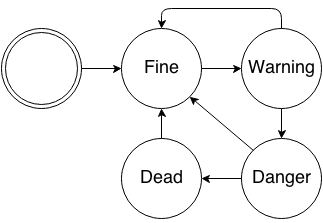
\includegraphics[scale=0.5]{state}
	\caption{State diagram of heartbeat state flow}
	\label{fig:hbstate}
\end{figure}

\subsection{Adding Hosts}

Adding hosts is no longer on the home page to make room for more hosts and because adding a host is not such a common operation that it needs to be on the home page.
In the case of PiCloud the add host form should be used to add the hosts to their corresponding towers and then left alone indefinitely until more Raspberry Pis are added to the PiCloud for example.
So instead of having the form on the home page, the form is on a separate page accessed by the plus icon in the top right of the home page (see figure \ref{fig:rmtCurrent}).

Next to this are links to the PiCloud website, since they were the ones to request the creation of this software, and a link to the GitHub page of \emph{rmt} since, as previously stated, the project will be made open source, and this provides an easy way for the user to find, and potentially contribute to, the project.

\begin{figure}[t]
	\centering
	\setlength\fboxsep{0pt}
	\setlength\fboxrule{0.5pt}
	\fbox{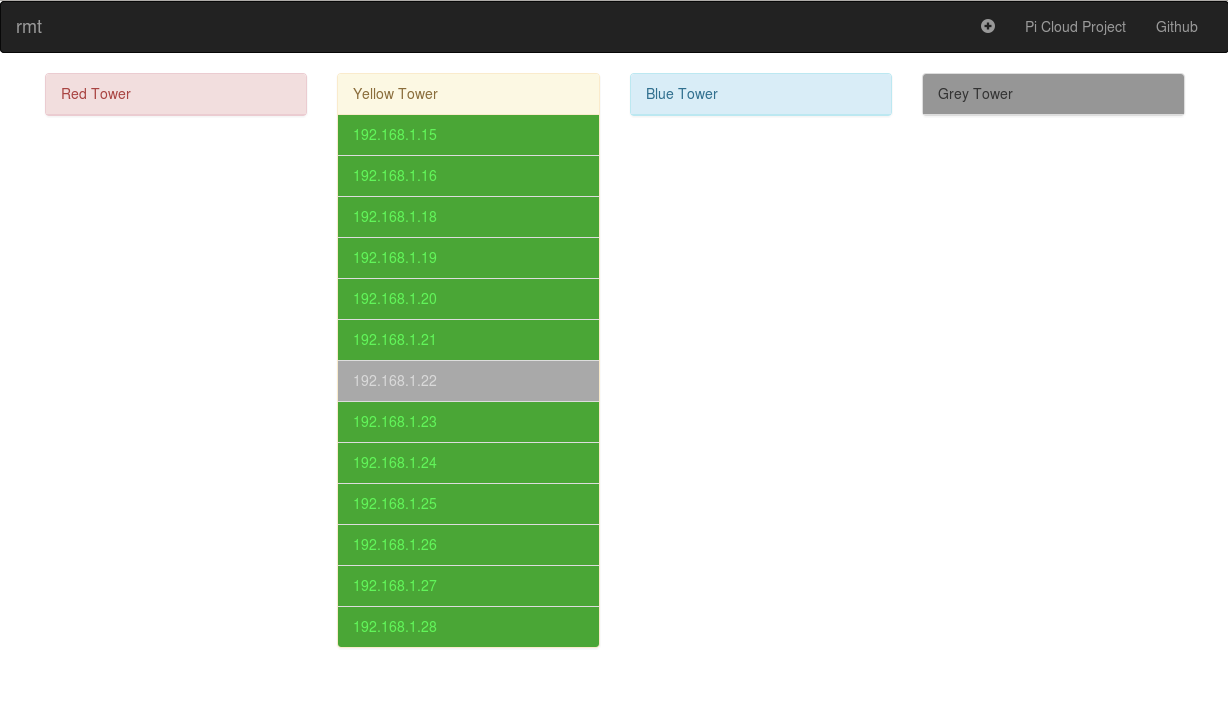
\includegraphics[width=0.8\textwidth]{rmtCurrent}}
	\caption{\emph{rmt}: home page}
	\label{fig:rmtCurrent}
\end{figure}

\begin{figure}[t]
	\centering
	\setlength\fboxsep{0pt}
	\setlength\fboxrule{0.5pt}
	\fbox{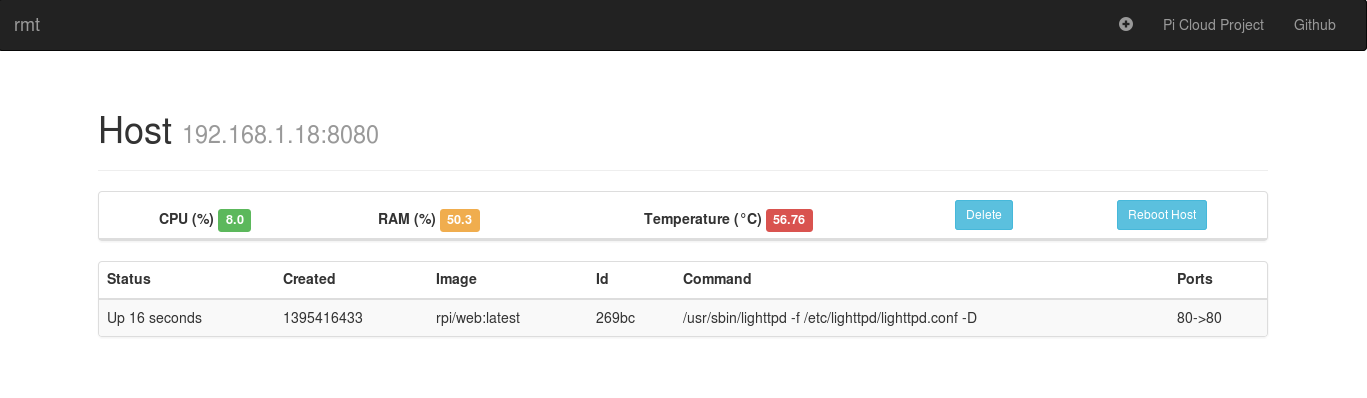
\includegraphics[width=0.8\textwidth]{rmtHostsCurrent}}
	\caption{\emph{rmt}: host page}
	\label{fig:rmtHostCurrent}
\end{figure}

\subsubsection{Host Page}

The design of the host page is somewhat inspired by the interface of Shipyard and DockerUI in that the table displayed shows similar fields.
Shipyard's container page (figure \ref{fig:shipyardContainers}) shows the Host field which \emph{rmt}'s host page does not need since this is already stated in the heading, and it shows the full ID of each container.
In \emph{rmt} the ID of the container is shortened to just five characters as this seemed sufficient to identify any containers running on a given host since, due to the Raspberry Pi's lack of resources, the number of containers actually able to run on any given Pi at once was so low as to be able to identify each container by the first five characters.
Additionally, the ``Description'' field seen in Shipyard's containers page was not available in the version of docker being used by PiCloud, so is not shown in \emph{rmt}'s host page.

The host page's container table actually more closely resembles DockerUI's containers table, shown in figure \ref{fig:dockerUiContainers}, though in a slightly different order and with fewer fields.
Admittedly the ``Status'' field in DockerUI is much more user-friendly with different labels to give more visual feedback to the user of the status of each container, however \emph{rmt} displays more fields, giving a better impression of what the containers are with the inclusion of the image name, and ports used in the case of running webservers.

\begin{figure}[t]
	\centering
	\setlength\fboxsep{0pt}
	\setlength\fboxrule{0.5pt}
	\fbox{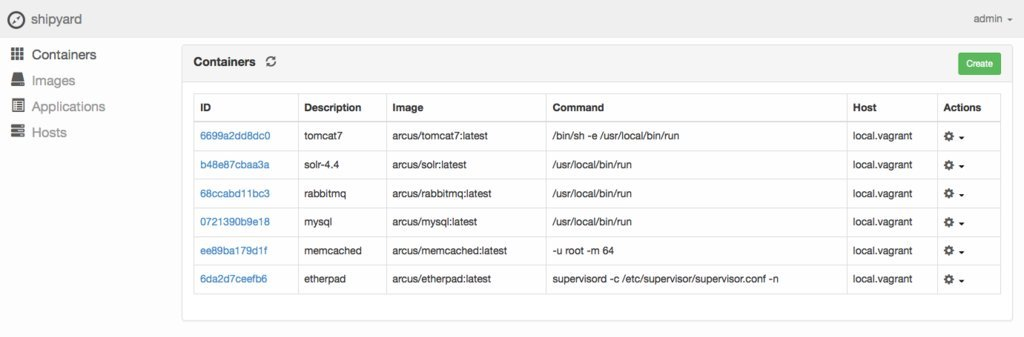
\includegraphics[width=0.8\textwidth]{shipyardContainers}}
	\caption{Containers page in Shipyard}
	\label{fig:shipyardContainers}
\end{figure}

By making the header, ``Host'', the user is reminded of where they are in the context of the system, and the sub-heading shows the user which host it is that they are viewing.
This includes the port of the client because there could feasibly be more than one client running on the same host.
This is entirely up to the systems administrator of the hosts but having more than one running instance of \verb%rmt_client% could add some redundancy to the host.

Labels throughout the system follow a colour scheme similar to that of the heartbeat states described earlier and are similarly configurable.

Buttons throughout the system are represented by Bootstrap's \verb%btn-info% class which is a light blue colour, making it visually distinctive to the status labels for CPU, RAM, and Temperature indicators, and the heartbeat states.

